\chapter{Taxonomy for Image Processing: Image types and algorithms}
\label{chap:image.algorithms.taxonomy}

\lettrine[lines=2]{I}{n} this thesis, we have pursued research into how to apply all those new generic facilities from
the C++ language into the Image processing area. This allows us to test them in a practical way on our predilection area
while remembering our past work, both success and failures in this matter. However, as we saw in the previous Chapter
(Generic programming (genericity)), birthing concepts from code is something that is done in an emerging way.
Henceforth, the first work will be to do an inventory of all existing image algorithms as well as an inventory of all
image processing algorithms (both basic and more complex) we can think of. This way, we will notice behavior patterns
emerging from similar image types or similar algorithms. We will then be able to extract behavioral patterns from this
inventory in order to produce a full taxonomy in the form of a framework of concepts related to image processing. This
chapter is structured as followed. First we will study how to extract behavioral pattern from a simple algorithm in
order to refine it into one or multiple concepts. Second we will study the theory set behind image types, their
conjunctions, disjunctions. We will also produce an inventory of image processing algorithms limited to mathematical
morphologies that we will leverage for the final step. Third, we will study the intrinsic genericity of algorithms to
produce canvas taking advantage of properties (linked to the types). Finally, we will study behavioral patterns, related
to the pre-established inventory of algorithms, in the form of a taxonomy engrave into a framework of concepts related
to image processing.

\section{Rewriting an algorithm to extract a concept}
\label{sec:rewriting}

\subsection{Gamma correction}
\label{subsec:gamma}

Let us take the gamma correction algorithm as an example. The naive way to write this algorithm can be:

\begin{minted}[linenos]{C++}
template <class Image>
void gamma_correction(Image& ima, double gamma)
{
  const auto gamma_corr = 1.f / gamma;

  for (int x = 0; x < ima.width(); ++x)
    for (int y = 0; y < ima.height(); ++y)
    {
      ima(x, y).r = 256.f * std::pow(ima(x, y).r / 256.f, gamma_corr);
      ima(x, y).g = 256.f * std::pow(ima(x, y).g / 256.f, gamma_corr);
      ima(x, y).b = 256.f * std::pow(ima(x, y).b / 256.f, gamma_corr);
    }
}
\end{minted}

\noindent This algorithm here performs the transformation correctly, but it also makes a lot of hypotheses. Firstly, we
suppose that we can write in the image via the \texttt{=} operator (l.9--11): it may not be true if the image is sourced
from a generator function. Secondly, we suppose that we have a 2D image via the double loop (l.6--7). Finally, we
suppose we are operating on 8bits range (0--255) RGB via \texttt{'.r'}, \texttt{'.g'}, \texttt{'.b'} (l.9--11). Those
hypotheses are unjustified. Intrinsically, all we want to say is \blockquote{\emph{For each value of \texttt{ima}, apply
    a gamma correction on it}}. Let us proceed to make this algorithm the most generic possible by lifting those unjustified
constraints one by one.



\paragraph{Lifting RGB constraint:}
First, we get rid of the 8bits color range (0--255) RGB format requirement. The loops become:

\begin{minted}{C++}
  using value_t = typename Image::value_type;

  const auto gamma_corr = 1.f / gamma;
  const auto max_val = std::numeric_limits<value_t>::max();

  for(int x = 0; x < ima.width(); ++x)
    for(int y = 0; y < ima.height(); ++y)
      ima(x, y) = max_val * std::pow(ima(x, y) / max_val, gamma_corr);
\end{minted}

\noindent By lifting this constraint, we now require the type Image to define a nested type\\
\texttt{Image::value\_type} (returned by \texttt{ima(x, y)}) on which \texttt{std::numeric\_limits} and
\texttt{std::pow} are defined. This way the compiler will be able to check the types at compile-time and emit warning
and/or errors in case it detects incompatibilities. We are also able to detect it beforehand using a
\texttt{static\_assert} for instance.1



\paragraph{Lifting bi-dimensional constraint:}
Here we need to introduce a new abstraction layer, the \emph{pixel}. A \emph{pixel} is a couple \((point, value)\). The
double loop then becomes:

\begin{minted}{C++}
  for (auto&& val : ima.values())
    val = max_val * std::pow(val / max_val, gamma_corr);
\end{minted}

\noindent This led to us requiring that the type \emph{Image} requires to provide a method \texttt{Image::pixels()} that
returns \emph{something} we can iterate on with a range-for loop: this \emph{something} is a \emph{Range} of
\emph{Pixel}s. This \emph{Range} is required to behave like an \emph{iterable}: it is an abstraction that provides a way
to browse all the elements one by one. The \emph{Pixel} is required to provide a method \texttt{Pixel::value()} that
returns a \emph{Value} which is \emph{Regular}~(see \cref{term:regular}). Here, we use \texttt{auto\&\&} instead of
\texttt{auto\&} to allow the existence of proxy iterator (think of \texttt{vector<bool>}). Indeed, we may be iterating
over a lazy-computed view~\cref{chap:image_views}.



\paragraph{Lifting writability constraint:}
Finally, the most subtle one is the requirement about the \emph{writability} of the image. This requirement can be
expressed directly via the new C++20 syntax for \emph{concepts}. All we need to do is changing the template declaration
by:

\begin{minted}{C++}
template <WritableImage Image>
\end{minted}

\noindent In practice the C++ keyword \texttt{const} is not enough to express the \emph{constness} or the
\emph{mutability} of an image. Indeed, we can have an image whose pixel values are returned by computing \(cos(x+y)\)
(for a 2D point). Such an image type can be instantiated as \emph{non-const} in C++ but the values will not be
\emph{mutable}: this type will not model the \emph{WritableImage} concept.



\paragraph{Final version}

\begin{minted}{C++}
template <WritableImage Image>
void gamma_correction(Image& ima, double gamma)
{
  using value_t = typename Image::value_type;

  const auto gamma_corr = 1 / gamma;
  const auto max_val = numeric_limits<value_t>::max();

  for (auto&& pix : ima.pixels())
    pix.value() = std::pow((max_val * pix.value()) / max_val, gamma_corr);
}
\end{minted}

\noindent When re-writing a lot of algorithms this way: lifting constraints by requiring behavior instead, we are able
to deduce what our \emph{concepts} needs to be. The real question for a \emph{concept} is: \blockquote{\emph{what
    behavior should be required?}}



\subsection{Dilation algorithm}
\label{subsec:dilation}

To show the versatility of this approach, we will now attempt to deduce the requirements necessary to write a classical
\emph{dilate} algorithm. First let us start with a naive implementation:

\begin{minted}[linenos]{C++}
template <class InputImage, class OutputImage>
void dilate(const InputImage& input_ima, OutputImage& output_ima)
{
  assert(input_ima.height() == output_ima.height()
    && input_ima.width() == output_ima.width());

  for (int x = 2; x < input_ima.width() - 2; ++x)
    for (int y = 2; y < input_ima.height() - 2; ++y)
    {
      output_ima(x, y) = input_ima(x, y)
      for (int i = x - 2; i <= x + 2; ++i)
        for (int j = y - 2; j <= y + 2; ++j)
          output_ima(x, y) = std::max(output_ima(x, y), input_ima(i, j));
    }
}
\end{minted}

\noindent Here we are falling into the same pitfall as for the \emph{gamma correction} example: there are a lot of
unjustified hypotheses. We suppose that we have a 2D image (l.7--8), that we can write in the \texttt{output\_image}
(l.10, 13). We also require that the input image does not handle borders, (c.f. loop index arithmetic l.7--8, 11--12).
Additionally, the \emph{structuring element} is restricted to a \(5 \times 5\) window (l.11--12) whereas we may need to
dilate via, for instance, a \(11 \times 15\) window, or a sphere. Finally, the algorithm does not exploit any potential
properties such as the \emph{decomposability} (l.11--12) to improve its efficiency. Those hypotheses are, once again,
unjustified. Intrinsically, all we want to say is \blockquote{For each value of \texttt{input\_ima}, take the maximum of
  the \(X \times X\) window around and then write it in \texttt{output\_ima}}.

To lift those constraints, we need a way to know which kind of \emph{structuring element} matches a specific algorithm.
Thus, we will pass it as a parameter. Additionally, we are going to lift the first two constraints the same way we did
for \emph{gamma correction}:

\begin{minted}{C++}
template <Image InputImage, WritableImage OutputImage, StructuringElement SE>
void dilate(const InputImage& input_ima, OutputImage& output_ima, const SE& se)
{
  assert(input_ima.size() == output_ima.size());

  for(auto&& [ipix, opix] : zip(input_ima.pixels(), output_ima.pixels())
  {
    opix.value() = ipix.value();
    for (const auto& nx : se(ipix))
      opix.value() = std::max(nx.value(), opix.value());
  }
}
\end{minted}

\noindent We now do not require anything except that the \emph{structuring element} returns the neighbors of a pixel.
The returned value must be an \emph{iterable}. In addition, this code uses the \texttt{zip} utility which allows us to
iterate over two ranges at the same time. Finally, this way of writing the algorithm allows us to delegate the issue
about the border handling to the neighborhood machinery. Henceforth, we will not address this specific point deeper in
this paper.

\subsection{Concept definition}
\label{subsec:concept}

The more algorithms we analyze to extract their requirements, the clearer the \emph{concepts} become. They are slowly
appearing. Let us now attempt to formalize them. The formalization of the \emph{concept Image} from the information and
requirements we have now is shown in~\cref{table:concept.definitions} for the required type definitions and
in~\cref{table:concept.expressions} for the required valid expressions.

\begin{table}[htbp]

  \begin{scriptsize}
    \texttt{Let \emph{Ima} be a type that models the concept \emph{Image}. Let \emph{WIma} be a type that models the
      concept \emph{WritableImage}. Then \emph{WIma} inherits all types defined for \emph{Image}. Let \emph{SE} be a
      type that models the concept \emph{StructuringElement}. Let \emph{DSE} be a type that models the concept
      \emph{Decomposable}. Then \emph{DSE} inherits all types defined for \emph{StructuringElement}. Let \emph{Pix} be a
      type that models the concept \emph{Pixel}. Then we can define:}

    \smallskip
    \begin{tabular}{l|l|l|l|}
      \cline{2-4}
                                                   & \thead{Definition }               &
      \thead{Description}                          & \thead{Requirement}                                      \\
      % Image
      \cline{1-4}
      \multicolumn{1}{|c|}{\multirow{3}{*}{Image}} & \texttt{Ima::const\_pixel\_range} & \makecell[l]{type of
        the range to iterate over
      \\ all the constant pixels} & \makecell[l]{models the concept \\
        \emph{ForwardRange}}
      \\
      \cline{2-4}
      \multicolumn{1}{|c|}{}                       & \texttt{Ima::pixel\_type}         & type of a pixel
                                                   & models the concept \emph{Pixel}                          \\
      \cline{2-4}
      \multicolumn{1}{|c|}{}                       & \texttt{Ima::value\_type}         & type of a value
                                                   & models the concept \emph{Regular}                        \\
      \cline{1-4}
      % Writable Image
      \multicolumn{1}{|c|}{\makecell[l]{Writable
      \\ Image}} & \texttt{WIma::pixel\_range} & \makecell[l]{type of the range to iterate over
      \\ all the non-constant pixels} & \makecell[l]{models the concept \\
        \emph{ForwardRange}}
      \\
      \cline{1-4}
      % StructuringElement \multicolumn{1}{|c|}{StructuringElement} &  &  & \\
      %  \cline{1-4} Decomposable \multicolumn{1}{|c|}{Decomposable} &  &  & \\
      %  \cline{1-4}
    \end{tabular}
  \end{scriptsize}
  \smallskip

  \caption{Concepts formalization: definitions}
  \label{table:concept.definitions}
\end{table}


\begin{table}[htbp]

  \begin{scriptsize}
    \texttt{Let \emph{cima} be an instance of \emph{const Ima}. Let \emph{wima} be an instance of \emph{WIma}. Then all
      the valid expressions defined for \emph{Image} are valid for \emph{WIma}. Let \emph{cse} be an instance of
      \emph{const SE}. Let \emph{cdse} be an instance of \emph{const DSE}. Then all the valid expressions defined for
      \emph{StructuringElement} are valid for \emph{const DSE} Let \emph{cpix} be an instance of \emph{const Pix}. Then
      we have the following valid expressions:}

    \smallskip
    \begin{tabular}{l|l|l|l|}
      \cline{2-4}
                                         & \thead{Expression}                              & \thead{Return Type} &
      \thead{Description}                                                                                          \\
      \cline{1-4}
      % Image
      \multicolumn{1}{|c|}{Image}        & \texttt{cima.pixels()}                          &
      \texttt{Ima::const\_pixel\_range}  & \makecell[l]{returns a range of constant pixels
      \\ to iterate over it} \\
      \cline{1-4}
      % Writable Image
      \multicolumn{1}{|c|}{\makecell[l]{Writable
      \\ Image}} &\texttt{wima.pixels()} & \texttt{WIma::pixel\_range}       & \makecell[l]{returns a range of
      pixels                                                                                                       \\ to iterate over it} \\
      \cline{1-4}
      % StructuringElement
      \multicolumn{1}{|c|}{\makecell[l]{Structuring
      \\ Element}} &\texttt{cse(cpix)} & \texttt{WIma::pixel\_range}       & \makecell[l]{returns a range of
        the neighboring
      \\ pixels to iterate over it} \\
      \cline{1-4}
      % Decomposable
      \multicolumn{1}{|c|}{Decomposable} & \texttt{cdse.decompose()}                       &
      \texttt{implementation defined}    & \makecell[l]{ returns a range of structuring
      \\ elements to iterate over it} \\
      \cline{1-4}
    \end{tabular}
  \end{scriptsize}
  \smallskip

  \caption{Concepts formalization: expressions}
  \label{table:concept.expressions}
\end{table}

The \emph{concept Image} does not provide a facility to write inside it. To do so, we have refined a second
\emph{concept} named \emph{WritableImage} that provides the necessary facilities to write inside it. We say
\blockquote{\emph{WritableImage} refines \emph{Image}}.

The \emph{sub-concept ForwardRange} can be seen as a requirement on the underlying type. We need to be able to browse
all the pixels in a forward way. Its \emph{concept} will not be detailed here as it is very similar to \emph{concept} of
the same name~\parencite{niebler.2018.mergingranges,niebler.2018.deepranges} (soon in the STL). Also, in practice, the
\emph{concepts} described here are incomplete. We would need to analyze several other algorithms to deduce all the
requirements so that our \emph{concepts} are the most complete possible. One thing important to note here is that to
define a simple \emph{Image concept}, there are already a large amount of prerequisites:
\label{term:regular}\emph{Regular}, \emph{Pixel} and \emph{ForwardRange}. Those \emph{concepts} are basic but are also
tightly linked to the \emph{concept} in the STL~\parencite{carter.2018.concepts}. We refer to the STL \emph{concepts} as
\emph{fundamental concepts}. \emph{Fundamentals concepts} are the basic building blocks on which we work to build our
own \emph{concepts}. We show the C++20 code implementing those \emph{concepts} in~\cref{code:concept.cpp20}.

\begin{figure}[htbp]

  \begin{minipage}[l]{0.48\linewidth}
    \begin{minted}{C++}
template <class Ima>
concept Image = requires {
    typename Ima::value_type;
    typename Ima::pixel_type;
    typename Ima::const_pixel_range;
  } && Regular<Ima::value_type>
  && ForwardRange<Ima::const_pixel_range>
  && requires(const Ima& cima) {
    { cima.pixels() }
      -> Ima::const_pixel_range;
  };

template <class I>
using pixel_t = typename I::pixel_type;
template <class SE, class Ima>
concept StructuringElement = Image<Ima>
  && requires(const SE& cse,
       const pixel_t<Ima> cpix){
    { se(cpix) } -> Ima::const_pixel_range;
  };
\end{minted}
  \end{minipage}
  \hfill
  \begin{minipage}[r]{0.48\linewidth}
    \begin{minted}{C++}
template <class WIma>
concept WritableImage = requires Image<WIma>
  && requires {
    typename WIma::pixel_range;
  } && ForwardRange<WIma::pixel_range>
  && ForwardRange<WIma::pixel_range,
       WIma::pixel_type>
  && requires(WIma& wima) {
    { wima.pixels() } -> WIma::pixel_range;
  };

template <class DSE, class Ima>
concept Decomposable =
  StructuringElement<DSE, Ima>
  && requires(const DSE& cdse) {
    { cdse.decompose() }
      -> /*impl. defined*/;
  };
\end{minted}
  \end{minipage}

  \caption{Concepts in C++20 codes}
  \label{code:concept.cpp20}
\end{figure}


\section{Image types viewed as Sets: version, specialization \& inventory}
\label{sec:image.set}

Achieving true genericity in a satisfactory way is a complex problem that has components of different levels. The first
goal is to natively support as many sets of image type as possible. Natively means that there is no need for a
conversion from one type to a super-type under the hood. The second step is to support an abstraction layer above the
underlying data type for each pixel. Indeed, the structure of an image is decorrelated from the underlying data type.
The third step is to write image processing algorithms for each set of image type. Fourthly, the performance trade-off
shall be negligible if not null. Finally, the final step is to provide a high degree of friendliness for the end user.
Ease of use is always to be considered, as notation (as in writting code) is a tool of
thought~\parencite{iverson.2007.notation}. Indeed, ``By relieving the brain of all unnecessary work, a good notation
sets it free to concentrate on more advanced problems, and in effect increases the mental power of the
race.''~\parencite{cajori.1993.history}.

Considering the available options to achieve our goal, the parametric polymorphism approach is the way to go. This
allows the implementer to design image types and algorithms with behavior in mind. To illustrate this remark, let us
consider the set of supported set of image types shown in~\cref{fig:image.version.vs.specialization}. We usually refer
to different image families as subtype. Indeed, an image with a LUT is subtype of the (global) Image type. This notion
of sub-typing is important because it may be abstracted behind an interface. A user can manipulate an image type without
knowing its specific subtype. This induces that the sub-typing facility may be handled internally in the library with
dynamic dispatching code (with runtime overhead). Each image processing library has its own way of handling sub-typing.
More generally, the model used to handle it is previously described in~\cref{subsec:different.approaches}. Indeed,
subtypes are handled the same way as their super-type but the fact that they have additional properties the algorithms
can take advantage of.

% \begin{figure}[htbp]
%   \centering
%   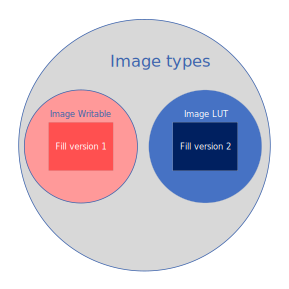
\includegraphics[width=.5\linewidth]{../figures/fill_version_diagram}
%   \caption{Diagram of the two versions of the fill algorithm.}
%   \label{fig:fill.version.diagram}
% \end{figure}

To implement a basic image algorithm such as \texttt{fill} there really are two distinct ways of writing it. For the set
of images type whose data type is encoded into each pixel, one must traverse the image and set each pixel's color to the
new one. However, for the set of images type whose data type is encoded in a look-up table, one only has to traverse the
look-up table to set each color to the new one. This translates into two distinct algorithms shown
in~\cref{fig:traverse.vs.LUT}. We can represent the diagram outlining that those two algorithms are two distinct
versions in~\cref{fig:image.version.vs.specialization}.

\begin{figure}[htbp]
  \centering
  \subfloat[Writable image fill algorithm]{
    \(fill(I, v)\colon \forall{p}\in\mathcal{D}, I(p) = v\)
  }
  \hfil
  \subfloat[Image LUT fill algorithm]{
    \(fill(I, v)\colon \forall{i}\in I.LUT, i = v\)
  }

  \caption{Comparison of implementation of the \texttt{fill} algorithm for two
    families of image type.}
  \label{fig:traverse.vs.LUT}
\end{figure}

More generally, we consider that the set of image type is formed of several subsets of image types. In the example there
are two subsets: images whose pixels are writable and images whose data type are ordered in a look-up table. \emph{For
  each one of these subsets, if there is a way to implement an algorithm then we have a \emph{version} of this algorithm}.

Sometimes, it is possible to take advantage of a property on a particular image set, that may be correlated to an
external data, to write the algorithm in a more efficient way. When those properties are linked to the types, it is
called algorithm \emph{specialization}~\parencite{jarvi.2006.specialization-article}. For instance, when considering a
dilation algorithm, if the structuring element (typically the disc) is decomposable then we can branch on an algorithm
taking advantage of this opportunity: decompose the dilation disc into small vectors and apply each one of them on the
image through multiple passes. The speed-up comparing to a single pass with a large dilation disc is really significant
(illustrated in~\cref{fig:gen.bench.square.disc}). The code in~\cref{fig:dilation.specialization.alg.diagram} illustrate
how an algorithm can be written to take advantage of the structuring element's decomposability property. The algorithm
will first decompose the structuring element into smaller 1D periodic lines. It will then recursively call itself with
those lines to do the multi-pass and thanks to known optimizations on periodic
lines~\parencite{vanherk.1992.localminmax}, it will be much faster. The dispatch diagram outlining the different
specialization of the dilation algorithm used is show alongside in~\cref{fig:dilation.specialization.alg.diagram}.

\begin{figure}[htbp]
  \begin{minipage}[l]{0.48\linewidth}
    \begin{minted}{C++}
template <Image Img, StructuringElement SE>
auto dilate(Img img, SE se) {
  if (se.is_decomposable()) {
    lst_small_se = se.decompose();
    for (auto small_se : lst_small_se)
      img = dilate(img, small_se) // Recursive call
    return img;
  } else if (is_pediodic_line(se))
    return fast_dilate1d(img, se) // Van Herk's algorithm;
  else
    return dilate_normal(img, se) // Classic algorithm;
}
\end{minted}
  \end{minipage}
  \hfill
  \begin{minipage}[r]{0.48\linewidth}
    \centering
    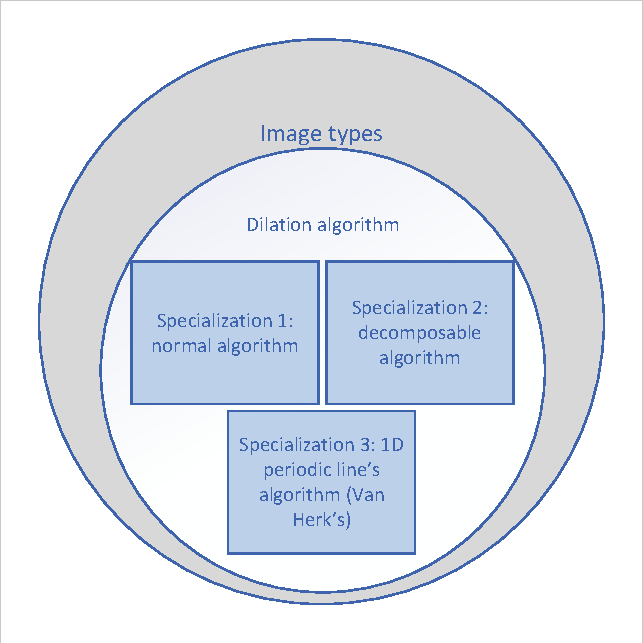
\includegraphics[scale=0.5]{../figures/dilation_specialization_diagram}
  \end{minipage}
  \caption{Dilate algorithm (left) with decomposable structuring element and its specialization diagram (right).}
  \label{fig:dilation.specialization.alg.diagram}
\end{figure}

The~\cref{fig:image.version.vs.specialization} shows how an algorithm specialization may exist in a set of algorithms
version. In this figure there exists a specialization of algorithms when it is known that the data buffer has the
following property: its memory is contiguous. This implies that, for example, an algorithm like \texttt{fill} can be
implemented using low level and fast primitives such as \texttt{memset} to increase its efficiency.

\begin{figure}[htbp]
  \centering
  \subfloat[Different versions of \emph{fill} algorithm]{
    \includegraphics[width=1.9in]{../figures/image_version}
  }%
  \hfil
  \subfloat[Specialization existing within a version]{
    \includegraphics[width=2.9in]{../figures/image_version_specialization}
  }%
  \caption{Set of algorithm version (a) and its specialization existing within a version (b).}
  \label{fig:image.version.vs.specialization}
\end{figure}

Making a full inventory of image types is not possible as there are many families of image types, each family may
intersect with each other, images may have some particular properties at some points, those properties may appear in
several families of image types. We can nonetheless cite a few to illustrate our points. There exists image-type whose
values are cubical complexes~\parencite{ziou.2002.cubical-complex} or layered as hexagonal or triangular grid instead of
square grids (such as meshes), that are represented as graphs~\parencite{meyer.2009.ismm}, etc. All of those interleaves
with different research areas (computer vision for meshes, topological classification for complex
cells~\parencite{movn.20.cviu,allili.2001.cubical}, graph theory and hierarchy for image
graphs~\parencite{carlinet.2014.tip,carlinet.2015.tip,perret.2019.higra}). Finally, this image type inventory does not
help when it comes to designing an image processing library. Instead, what helps is making an inventory of image
processing algorithms as well as what properties those algorithms can leverage to speed up their execution.

By making the inventory of image processing algorithms (limited to mathematical morphology), we distinguish three main
types of image processing algorithms. The first one are the pixel-wise algorithms. Those algorithms are the basic
pixel-wise transformation. They are the base of any image processing toolkit. Indeed, being able to extract the green or
red color channel of an image is mandatory. Thresholding as well as the previously seen gamma correction are such
algorithm. The second one are the local algorithms. Those algorithms perform transformations by considering all the
neighboring pixels around a given pixel. In order to operate, those algorithms need additional data in the form of
image's extension (defining border's behavior) and structuring element (disc, rectangle around the considered pixel).
Such algorithms are widely used in mathematical morphology. Dilation, erosion, closing, opening, gradient, rank filter
are all local algorithms, as well as stencil-type algorithms such as union-find, max-tree or skeletonize. Finally, the
third set of image processing algorithms is the global one. This set contains algorithms where computing the current
pixel requires to knowledge about what was previously computed for the previous pixels. Chamfer distance transform,
labeling, watershed, hierarchy structures related algorithms are in this category.


\section{Generic aspect of algorithm: canvas}
\label{sec:canvas}

Genericity is always referred to with this sentence \blockquote{write once, work for every type, run everywhere}.
However, very quickly we learned that the \emph{run} aspect can be a combination of:
\begin{itemize}
  \item as fast as possible on a single CPU unit;
  \item as fast as possible on thanks to using many CPU units;
  \item as fast as possible on thanks to using many GPU units;
  \item as fast as possible on thanks to using many computers (cloud) and their CPU/GPU units.
\end{itemize}
How do we decide what is the most efficient way to do? There is no simple answer to this question, but we can start by
studying the morphology of algorithms with two goals in mind: (i) find what can be parallelized/distributed and (ii)
find one or several algorithms' abstraction. Indeed, in image processing there are a lot of common patterns when one
looks at algorithms implementations, the most famous being \emph{for all pixels of an image, do something to each
  pixel}. But there are other more high-level similarities that we can leverage to have more generic algorithm. Let us
first study the different programmatic model there are commonly used to process images.

\FIXME{Rework these 3 paragraphs}

\paragraph{The pipeline} It is the classic way of doing the work. It consists of an imbrication of different operators
(algorithms) taking as input one or several images, maybe additional data as well (such as labels, adjacency map, etc.)
in order to process the data \blockquote{from left to right}. The result will show at the end of the pipeline and the
optimization opportunities are located inside the smaller operators and in the form of correctly managing data (no
useless copies, locality, etc.)

\paragraph{Kernels and tiling} They are the trendy way of the last decade. It consists in breaking the original image
into small tiles in order to feed those tiles into a massively multicore GPU (via CUDA,
Halide~\parencite{ragankelley.2013.halide}). Processing will happen concurrently on those core, but it is costly to swap
contents inside those GPU from the RAM memory. It's then preferred to design pipeline for those tiles so that the work
directly happens on each core to minimize the number of back and forth copies from the RAM.

\paragraph{Cloud computing} It is a huge deal in image processing these last years as well, especially used in Deep
learning applications. Deep neural networks are usually executed on cluster of computer through network (cloud) and thus
are leveraging combinations of successive \emph{MapReduce}~\parencite{dean.2008.mapreduce} under the hood. They can also
be offloaded onto or local available computers, or directly locally available GPU hardware thanks to frameworks that are
dynamically dispatching the workload (such as
Tensorflow/Keras~\parencite{tensorflow.2015.whitepaper,chollet.2015.keras,gulli.2017.deep},
PyTorch~\parencite{paszke.2019.pytorch}, etc.).

In every case there is a notion of pipeline where the user pipe algorithms into each others in order to achieve a
result. Those algorithms can leverage all the heterogeneous resources (cloud, GPU, CPU) they can to \emph{map} the input
data. Algorithms will then finally aggregate the results (\emph{reduce}) to output them into another algorithm, or save
them, or display them. It is important to dissociate the route the data will go through and the processing pipeline
logic. Both have their own specificities. In this thesis, we make a parallel, at small scale, between processing
pipeline logic and image processing algorithms. First let us study two basic algorithms: dilation and erosion. The
Python code of such algorithm is naively be given in~\cref{code:erode.dilate}.

\begin{figure}[htbp]
  \centering
  \subfloat[Dilation]{
    \includegraphics[width=1.7in]{../figures/dilation_code}
  }%
  \hfil
  \subfloat[Erosion]{
    \includegraphics[width=1.7in]{../figures/erosion_code}
  }%
  \caption{Dilate vs. Erode algorithms.}
  \label{code:erode.dilate}
\end{figure}

The algorithms are almost written the same way. The only change is the operation \emph{min} and \emph{max} when
selecting the value to keep. As such, we can easily see a way to factorize code by passing the operator as an argument.
The algorithms can then be rewritten as shown in~\cref{code:erode.dilate.factorized}. In this last example, we have one
piece of code which is in charge of abstracting the way an image is traversed: it is the canvas. We also have other
pieces of code which carry the logic of the operations, calling the canvas and providing the logic to apply from within
the canvas. This way of decomposing the code offers the opportunity of writing more specific heterogeneous logic for the
traversing code so that the other parts of the code that carry the operator logic remains unaware and unburdened of
possible implementation details.

\begin{figure}[htbp]
  \centering
  \subfloat[Local algorithm with custom operator]{
    \includegraphics[width=3.28in]{../figures/local_op_code}
  }%
  \vfil
  \smallskip
  \subfloat[Dilation (delegated)]{
    \includegraphics[width=1.64in]{../figures/local_op_dilation_code}
  }%
  \hfil
  \subfloat[Erosion (delegated)]{
    \includegraphics[width=1.64in]{../figures/local_op_erosion_code}
  }%
  \caption{New Dilate vs. Erode algorithms.}
  \label{code:erode.dilate.factorized}
\end{figure}

\subsection{Taxonomy and canvas}
\label{subsec.taxonomy.canvas}

This approach is very much compatible with the inventory of the algorithms we did in the previous~\cref{sec:image.set}.
Indeed, for the point-wise family of algorithms, it is hardly an issue as they can all be written in terms of
views~\cref{chap:image_views}. For the second family, which consists in all the local algorithm, they may be abstracted
behind an algorithm canvas where the user provides the work to do at each point of the algorithm. For instance, a single
pass local algorithm will always have shape given in~\cref{code:local.algorithm.canvas}. Finally, for third family which
consists in all the algorithm that propagate their computation while traversing the image. It is way less easy to
provide an algorithmic canvas as each algorithm has its own way to propagate changes curing its computation.

\begin{figure}[htbp]
  \centering
  \begin{minted}[linenos,xleftmargin=17pt,gobble=2]{python}
  def local_canvas(img, out, se):
    # do something before outer loop
    for pnt in img.points():
      # do something before inner loop
      for nx in se(pnt):
        # do something inner loop
      # do something after inner loop
    # do something after outer loop
  \end{minted}

  \caption{Local algorithm canvas.}
  \label{code:local.algorithm.canvas}
\end{figure}

This canvas can be customized to do a specific job, especially at the lines 2, 4, 6, 7 and 8. The user would then
provide callbacks and the canvas would do the job. This is especially useful when knowing that the canvas would handle
the border management (the user would provide a handling strategy like mirroring the image or filling it with a value).
The canvas would also take advantage of optimization opportunities (such as the decomposability of a structuring
element) that the user would probably forget, or not know, when first writing his local algorithm. Another advantage is
the opportunity to do more complex optimization such as parallelizing the execution or offloading part of the
calculation on a GPU. More generally, all optimization done through heterogeneous computing would be available by
default even if the user is not an area expert.

Despite all these advantages, one big disadvantage is the readability of the algorithm user-side. For instance, the
dilation algorithm is rewritten in~\cref{code:local.algorithm.dilate}.

\begin{figure}[htbp]
  \centering
  \begin{minted}{python}
def dilate(img, out, se):
  do_nothing = lambda *args, **kwargs: None

  def before_inner_loop(img, out, pnt):
    out(pnt) = img(pnt)

  def inner_loop(ipix, opix, nx):
    out(pnt) = max(out(pnt), img(nx))

  local_canvas(img, out, se,
    before_outer_loop = do_nothing,
    before_inner_loop = before_inner_loop,
    inner_loop        = inner_loop,
    after_inner_loop  = do_nothing,
    after_outer_loop  = do_nothing
  )
  \end{minted}

  \caption{Local algorithm canvas.}
  \label{code:local.algorithm.dilate}
\end{figure}

This way of thinking algorithms is far less readable than the classic way. The user does not see the loops happening,
and it can become very messy when several passes are happening (closing, opening, hit or miss, etc.)


\subsection{Heterogeneous computing: a partial solution, canvas}
\label{subsec:heterogeneous}

One of the key aspect driving genericity is performance. We still have the following mantra: \blockquote{write once,
  work for every type, run everywhere}. However, when considering the \emph{run} aspect, one has a lot to do. Indeed,
nowadays, leveraging the available resources to their maximum is long-standing issue. There are many ongoing works on
the subject, such as SyCL~\parencite{brown.2019.heterogeneous,wong.2019.heterogeneous} which is a standard for
heterogeneous computing model edited by Kronos. This standard currently has four implementations: Codeplay's
ComputeCpp~\parencite{codeplay.2021.computecpp}, Intel's LLVM/clang implementation~\parencite{intel-llvm.2021.sycl},
triSYCL~\parencite{xilinx.2021.triSYCL} led by Xilinx and hipSYCL~\parencite{aksel.2020.hipsycl} led by Heidelberg
University. There also exists smaller libraries such as Boost.SIMD~\parencite{esterie.2014.boostsimd} or even
VCL~\parencite{fog.2013.vcl} for easing how to write SIMD code. After taking some distance to study the subject, we can
infer that there are three main aspects to consider when optimizing performance.

The first one, the most important one is the algorithm to use in function of certain set of data. This aspect is covered
by the C++ language and its built-in genericity tool: template metaprogramming. Indeed, we select the most optimized
algorithm for a particular set of data.

The second one is the ability for the code to be understood by the compiler so that it can be further optimized during
the generation of the binary. Indeed, when compiling for the native architecture of a recent processor, one can use the
most recent assembly instructions to use wide vectorized registries (AVX512). The use of a recent compiler also brings
the help much needed.

Finally, the third aspect is not as trivial as the first two ones. It consists in studying the structure of an algorithm
to allow distributed computation. It also consists in studying the different architectures to select the most efficient
algorithm for a given architecture. Sometimes algorithm are friendly to be distributed on several processing units that
compute a part of the result concurrently. This is what we call parallelism. There exists several ways to take advantage
of parallelism. First there is the use of several CPU units on the host computer. Then there is the use of GPU units
working in combination with the CPU units to take advantage of the massive amount of core a graphic card can provide.
Finally, there is the use of cloud computing which consists in using several ``virtual'' computers, each of them
offering of CPU and GPU units in order to compute a result. One should be aware that each time we introduce a new layer
of abstraction, there is a cost to orchestrate the computation, send the input data and retrieve the results. It is thus
very important to study case by case what is needed. Some solutions exist that abstract away completely the hardware
through a DSL~\footnote{Domain Specific Language} such as Halide~\parencite{ragankelley.2013.halide}: the DSL compiler's
job will be to try very hard to make the most out of both the available (or targeted) hardware and the code. Those
solutions are not satisfactory for us as we want to avoid DSL and remain at code level. We are not developing a
compiler: we are working with it.

There is one true issue when studying parallel algorithm: it is whether they can be parallelized or not. Not all
algorithms can be parallelized. Some just intrinsically cannot, typically, algorithms that immediately need the result
at the previous iteration to compute the next iteration. There may exist specific ways to re-arrange a specific
algorithm, for instance, taking advantage of some algebraic property, in order to rewrite it in a parallelizable way,
but it is not trivial (on a per-algorithm basis), and not generic. As such, it is out of the scope of this thesis. What
interest us are the algorithms whose structure is an accumulation over a data type that can be defined as a monoid. We
assert that every algorithm that can be rewritten as an accumulation over a monoid can be parallelized and/or
distributed. This model that consists in distributing computation like an accumulation over a monoid data structure is
also call the map-reduce. This model has two steps: the distribution (map) and then the accumulation (reduce).

The map step will dispatch computation on subunits with small set of data. The reduce step will retrieve and accumulate
all those resulting data, as soon as they are ready.

The accumulation algorithm has this form:
\begin{minted}[linenos]{C++}
  template <class In, class T, class Op>
  auto accumulate(In input, T init, Op op)
  {
    for(auto e : input)
    {
      init = op(init, e);
    }
    return init;
  }
\end{minted}

The loop line 4 can be split into several calculation units which are going to be distributed, and then be accumulated
later once the units have finished their computation.

The issue left here is the monoid. What exactly is a monoid here? A monoid is a data structure which operates over a set
of values, finite or infinite. This data structure must provide a binary operation which is closed and associative.
Finally, this data structure must also provide a neutral element (aka the identity). Some trivial monoids comes to mind:
\begin{itemize}
  \item \emph{boolean}. For binary operation ``and'', identity is ``true'' whereas for binary operation ``or'', identity
        is ``false''.
  \item \emph{integer}. For binary operation \(-\) and \(+\), identity is \(0\) whereas for binary operation \(*\) and
        \(/\), identity is \(1\).
  \item \emph{string}. For concatenation, identity is empty string.
  \item \emph{optional} value (also known as monadic structure in Haskell programming language).
\end{itemize}
There are many more monoids, less trivial but very handy, such as the unsigned integer/max/0 set and the signed
integer/min/global max set.

This theory is extremely beneficial to image processing as the most commonly used algorithms, the local algorithms, can
all be written in the form of an accumulation over the pixels of an image. The fact that finding an identity for the
operation processed by the algorithm is often quite trivial led us to the idea of canvas. A canvas is a standard way to
write an iteration over an image which abstracts the underlying data structure. A canvas is a tool for the user to
provide its computation model based on events such as: \blockquote{entering inner loop} or \blockquote{exiting inner
  loop}. The user can then provide its operations as if he was writing his algorithm himself (restricted to the
accumulation model). As the maintainer of the library provides the canvas of execution, he can know also make change to
take advantage of it. For instance, computing a CUDA kernel at one point and dispatching it on GPU units is totally
within scope and transparent for the user of the library. Although there is a caveat: rewriting our algorithm in an
accumulation form and chunking it in fragments to feed to the canvas is definitely not intuitive. Indeed, we require our
user to change his way of thinking from the procedural paradigm to the event-driven paradigm. This approach is not new
and is used in other libraries such as Boost.Graph~\parencite{siek.2001.boostgraph} for similar purposes.
\citeauthor{dean.2019.monoids} talks about this recurring monoid pattern more in-depth in his
talk~\parencite{dean.2019.monoids}.

In image processing, we quickly come to identify \emph{local} algorithms, that reason about a group of pixel around a
given of coordinate. All those algorithms can be abstracted behind an accumulation of some sort, and they all have the
same morphology. Thus leading to the following abstraction:
\begin{minted}{C++}
template <class In, class Out, class SE, class T, class Op>
auto local_accumulate(In input, Out output, SE se, T init, Op op)
{
    auto zipped_imgs = ranges::view::zip(input.pixels(), output.pixels())
                                                  // (1)
    for(auto&& rows : ranges::rows(zipped_imgs))
    for(auto [px_in, px_out] : rows)
    {
        auto v = op(init, px_in.val());           // (2)
        for(auto nb : se(px_in))
        v = op(v, nb.val());                      // (3)
        px_out.val() = v;                         // (4)
      }
                                                  // (5)
  }
\end{minted}
From this code we can deduce some very useful and easy monoids by the following triplets:
\begin{itemize}
  \item \((type = boolean, operator = and, neutral = true)\) is a binary erosion
  \item \((type = boolean, operator = or, neutral = false)\) is a binary dilation
  \item \((type = unsigned integer, operator = max, neutral = 0)\) is a dilation
  \item \((type = signed integer, operator = min, neutral = global max)\) is an erosion
\end{itemize}

Now if we want to rewrite the \texttt{local\_accumulate} in an event driven paradigm, we need to identify the different
callbacks to expose our user on the call site. Especially, what will be of the callback parameters. There are five
callback events we have identified:
\begin{enumerate}
  \item before entering outer loop (no work is done)
  \item before entering inner loop (iteration over the pixel's neighbor)
  \item inner loop (actual operation to perform, result is accumulated)
  \item after exiting inner loop (iteration over the neighbor is over, what to do with the accumulated result?)
  \item after exiting outer loop (iteration over the image is over)
\end{enumerate}
\begin{minted}{C++}
template <class In, class Out, class SE, class T, class BeforeOuterLoopCB,
          class BeforeInnerLoopCB, class InnerLoopCB class AfterInnerLoopCB,
          class AfterOuterLoopCB>
auto local_accumulate(In input, Out output, SE se, T init,
                      BeforeOuterLoopCB bolCB, BeforeInnerLoopCB bilCB,
                      InnerLoopCB ilCB, AfterInnerLoopCB ailCB,
                      AfterOuterLoopCB aolCB)
{
  auto zipped_imgs = ranges::view::zip(input.pixels(), output.pixels()
  bolCB(input, output);                             // (1)
  for(auto&& row : ranges::rows(zipped_imgs))
    for(auto [px_in, px_out] : rows)
    {
      bilCB(px_out.val(), init, px_in.val())        // (2)
      for(auto nb : se(px_in))
        ilCB(px_out.val(), px_out.val(), nb.val())  // (3)
      ailCB(px_out.val(), init, px_in.val())        // (4)
    }
  aolCB(input, output)                              // (5)
}
\end{minted}
In this code, we can see that all the callbacks do not take the same type and/or number of parameters. Here is what the
call site would like if the user wants to perform a dilation:
\begin{minted}{C++}
local_accumulation(
  input,                                    // input image
  output,                                   // output image
  se,                                       // structuring element
  0,                                        // monoid's neutral element
  [](auto I, auto& O) { /* do nothing */ }, // (1) entering outer loop callback
  [](auto& o, auto init, auto in){          // (2) entering inner loop callback:
    o = std::max(init, in);                 // initialize with neutral element
  },
  [](auto& o, auto cur, auto nbh) {         // (3) inner loop callback:
    o = std::max(cur, nbh);                 // keep the local maximum
  },
  [](auto& o, auto init, auto in) {         // (4) exiting inner loop callback
    /* do nothing */
  },
  [](auto I, auto& O) { /* do nothing */ }  // (5) exiting outer loop callback
);
\end{minted}
It is very verbose and non-intuitive but hopefully, once the compiler optimize out the empty callbacks, the generated
code is as fast as a non-generic handwritten dilation.

\section{Library concepts: listing and explanation}
\label{sec:library.concepts}

Let us now delve into concepts related to the Image Processing area. Indeed, this domain has his specificities, and we
want to improve generic image processing library design by learning from our past experiments and working with new
techniques. The most basic usage of an image is the famous algebraic formula \(y = f(x)\) where \(y\) is a \emph{value}
generated by the \emph{image} \(f\) for the \emph{emph} \(x\). Aside from generating a value, an image can also
\emph{store} a value, as in \(f(x) = y\) where the value is \emph{assigned} to the image for a given point. Those
notions are the basis of our work and will drive the entire design.

\subsection{The fundamentals}

\label{subsec:fundamentals}

First, let us introduce the fundamental concepts deriving from the basis notion. The \emph{Value} concept is refined
into three distinct one in~\cref{table:concept.value.expressions}. There are the basic \emph{Value} but also the
\emph{ComparableValue} and the \emph{OrderedValue} which are useful when it comes to comparison or ordering algorithms.
The need behind those three concepts derives from the algorithms who need an ordering relation in order to function
properly. Most of mathematical morphology requires it. For instance, the ordering relation for a gray-scale image is
trivial whereas it is a field of research for colored (rgb-8bits) images.

The second fundamental brick is the concept of \emph{Point}, detailed in~\cref{table:concept.point.expressions} which is
a bit less open than the concept \emph{Value} as it must be totally ordered. Indeed, when accessing a value stored in an
image, whether it is about reading or mutating, it is important that there is only one accessed value.

Now we introduce an abstract way to represent this relation \(Value \times Point\): the Pixel. This is a well known
notion in image processing, and it represents a couple \((point, value)\). This abstraction layer is easy to move around
and contains facilities to read and mutate the pixel's value if possible. Indeed, not all pixels are able to mutate
their value. If the pixel is yielded by an image that only generates values on the fly then it cannot be mutated.
Henceforth, we introduce two new concepts: \emph{Pixel} and \emph{OutputPixel}
in~\cref{table:concept.pixel.definitions}. Those two concepts have a very similar interface described
in~\cref{table:concept.pixel.expressions}. They can both access the stored information: the point and the value. On top
of that, the \emph{OutputPixel} can mutate the value. When interacting with pixels, the user will want to be able to
write code as followed:
\begin{minted}{C++}
  auto pix = Pixel();     // Get a pixel
  auto val = pix.val();   // yield the pixel value
  auto pnt = pix.point(); // yield the pixel point
  pix.val() = 42;         // Assign a value
\end{minted}

We show how those three fundamental concepts interact with each other in the\\
diagram~\cref{fig:concept.pixel}.

\begin{figure}[htbp]
  \centering
  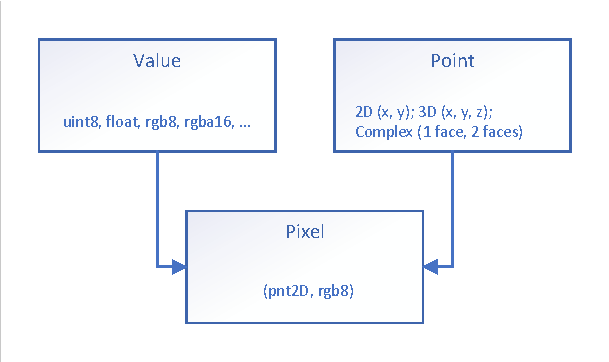
\includegraphics[width=.8\linewidth]{../figures/concepts/pixel}
  \caption{Pixel concept.}
  \label{fig:concept.pixel}
\end{figure}

Now we need a helper concept: the ranges.
Ranges~\parencite{niebler.2014.ranges,niebler.2018.ranges,niebler.2018.deepranges,niebler.2018.mergingranges} are a set
of concepts defined in the C++ standard library shipped with the ISO C++20 norm in 2020~\parencite{iso.2020.cpp}. They
allow the user to abstract away iterators to only iterate over one object: the range. This offers the user the
opportunity to migrate his source code from:
\begin{minted}{C++}
template <class IteratorBegin, class IteratorEnd>
void my_algorithm(IteratorBegin beg, IteratorEnd end)
{
  for(; beg != end; ++beg)
    // ...
}
\end{minted}
To:
\begin{minted}{C++}
template <class Range>
void my_algorithm(Range rng)
{
  for(auto e : rng)
    // ...
}
\end{minted}

In image processing, we refine further this concept by introducing multidimensional ranges (\emph{MDRange}). Indeed, in
image processing the user is used to write double loop to iterate over a bi-dimensional image. And abstracting away this
aspect under standard ranges induces performance loss. That is why we needed this concept to exist. A multidimensional
range can be split with a library function, \texttt{mln::ranges::rows(mdrng)} to fit the double-loop pattern and keep
its performance. This topic is tackle in-depth later in~\cref{subsec.range.traversing}. For now, let us consider
multidimensional ranges as an image processing extension for performance for the image traversing pattern. They are
defined in~\cref{table:concept.ranges.definitions} and their interface is the same as standard ranges, as seen
in~\cref{table:concept.ranges.expressions}. They are designed so that the user code looks like this:
\begin{minted}{C++}
  auto mdrng = MDRange(); // Get a multi-dimensional range of values
  auto rows = mln::ranges::rows(mdrng);
  for(auto row : rows) // double loop pattern
    for(auto val : row)
      // use(val)
\end{minted}

From an algebraic point of view, the definition of an image is not complete without considering a definition domain on
which it is defined. In image processing, the same rule applies. We cannot consider an image without considering the set
of points that are valid for this image. Henceforth, we must define the concept of \emph{Domain}
in~\emph{table:concept.domain.definitions}. The \emph{Domain} concept is refined into two sub-concepts which are
\emph{SizedDomain} and \emph{ShapedDomain}. This emphasis the chance of existence of possible infinite domain as
well as domains that may be defined over non-continuous intervals in space. This enables algorithms to require the
domain to have certain shape if needed. The domain behavior is described in~\cref{table:concept.domain.expressions}.

In practice, a domain is used to get information about the points constituting the image. Indeed, we can write code
like this:
\begin{minted}{C++}
  auto dom = Domain(); // Get a domain
  auto pnt = Point(..., ...); // Get a random point
  bool ret = dom.has(pnt); // Check wether the domain contains the point
  bool is_empty = dom.empty(); // Check wether the domain is empty
  auto dim = dom.dim(); // Yield the domain's dimension information
\end{minted}

We show how the concept \emph{Domain} flows from the previous concepts in the diagram shown in~\cref{fig:concept.domain}.

\begin{figure}[htbp]
  \centering
  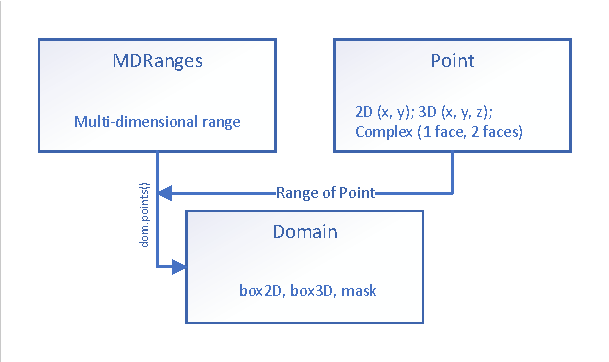
\includegraphics[width=.8\linewidth]{../figures/concepts/domain}
  \caption{Domain concept.}
  \label{fig:concept.domain}
\end{figure}

Now we have all the tools to introduce our main concept: \emph{Image}. As for \emph{Pixel}, we have the distinction over
image whose value can be mutated in a sub-concept named \emph{WritableImage}. These concepts are defined
in~\cref{table:concept.image.definitions.1}. In addition to this definition we can infer the behavior described
in~\cref{table:concept.image.expressions.1}. There are complicated requirements written in template metaprogramming code
and, in summary, they just require that the value types of the ranges returned by the member functions \texttt{pixels()}
and \texttt{values()} are the same as the value types declared in the parent image. In addition, we introduce two
facilities which are the member function \texttt{concretize()} and \texttt{ch\_value<V>()}. The first is a way to turn a
view into a concrete type. This will be seen more in-depth in~\cref{chap:image_views}. The last is a way to cast values
from one type to another. It forms a new image type whose underlying values will be returned after being converted to a
new value type. This last facility is extremely useful when one only wants to mutate the underlying type while keeping
all the other details about one type (such as the dimension). For instance, when working with labeling algorithm, we
know our algorithm will return an image similar to the input one except for the underlying type which will be the type
of the label. The following code shows how it is applied:
\begin{minted}{C++}
  using label_t = int; // label type

  template <class I> // Input image of type I
  auto my_labeling_algorithm(I input_image)
    -> image_ch_value_t<I, label_t> // Output image is Input image (I)
                                    // whose underlying type is label_t
  {
    // ...
  }
\end{minted}

We show the diagram building up the image concept from the previous concepts in~\cref{fig:concept.image}.

\begin{figure}[htbp]
  \centering
  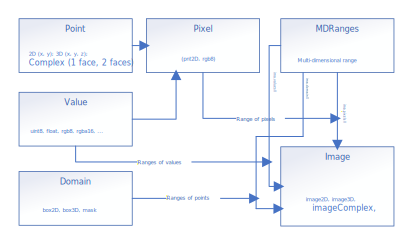
\includegraphics[width=.8\linewidth]{../figures/concepts/image}
  \caption{Image concept.}
  \label{fig:concept.image}
\end{figure}


\subsection{Advanced way to access image data}
\label{subsec:advanced}

While being able to iterate over ranges of pixels or values is good, we are still lacking fundamental facilities to
access an element directly from the image. In order to solve this predicament, first we need to define the concept of
\emph{Index} in~\cref{table:concept.index.expressions} which we will use afterwards. This is a very simple concept that
encapsulate an integral value. This value can be negative as we want to be able to do negative indexing in case our
image has an extension, c.f.~\cref{subsec:advanced}. The first advanced tool is represented as an \emph{IndexableImage}.
An element can be accessed simply by providing its index number. This concept is defined
in~\cref{table:concept.image.definitions.2}. This introduces a simple behavioral pattern described
in~\cref{table:concept.image.expressions.2}. With this concept, we are able to write code as followed:
\begin{minted}{C++}
  auto ima = IndexableImage(); // Get an indexable image
  int k = 15; // Get an index
  auto val = ima[k]; // Get the element at the index
  ima[k] = 255; // Mutate the element at the index
\end{minted}
Being able to traverse an image through indexes is especially useful for algorithms that are aware of the number of
elements in the image. We chose to be flexible with our indexing method (i.e. allowing signed indexes) not to fall into
the same pitfall as the C++ core language~\parencite{stroustrup.2019.signed-unsigned-mess}. Indeed, requiring that the
type \texttt{std::size\_t} is unsigned lead to loads of issues, the first one being a conversion issue when writing a
simple for-loop. Solving these issues lead to the appearance of new member function \texttt{.ssize()} (for signed size)
and the new type \texttt{std::ptrdiff\_t} to store the result of a subtraction between two \texttt{std::size\_t}.
Furthermore, in our specific area (image processing), it may be well-defined to access a buffer with negative indexes
when, for instance, we are accessing the value of the extension of an image. This is why our indexes are signed.

Additionally, we want to be able to access a value by providing a point, the same way as in the algebraic definition
\(val = image(point)\). To do so, we introduce the concept of accessibility through \emph{AccessibleImage}. This concept
is defined in~\cref{table:concept.image.definitions.3}. This introduces new behavior that is described
in~\cref{table:concept.image.expressions.3}. We can notice facilities specifically including bound checking. Indeed, we
suppose, for fast access, that the user is always picking element from the image's domain, but it is possible to bound
check elements if needed on access for specific usages. With this concept, we are now able to write code as followed:
\begin{minted}{C++}
  auto ima = AccessibleImage(); // Get an accessible image
  auto p = Point(); // Get a point
  auto val = ima(p); // Get a value from a point
  auto val = ima.at(p) // Same with no bound checking
  auto pix = ima.pixel(p) // Get a pixel from a point
  auto pix = ima.pixel_at(p) // Same with no bound checking
  ima(p) = 42; // Assign a value from a point
  ima.at(p) = 42; // Same with no bound checking
  ima.pixel(p).val() = 42; // Assign a pixel value from a point
  ima.pixel_at(p).val() = 42; // Same with no bound checking
\end{minted}
Being able to traverse an image through points is especially useful for algorithms relying on restricting/expanding
definition domain that are exclusively yielding points.

Once we know that an image is both \emph{indexable} and \emph{accessible} we can introduce new behaviors (described
in~\cref{table:concept.image.expressions.4}) that we put behind the concept of \emph{IndexableAndAccessibleImage}
defined in~\emph{table:concept.image.definitions.4}. This behavior is related to accessing index from points and vise
versa. Indeed, it is possible to now write such code:
\begin{minted}{C++}
  auto pnt = ima.point_at_index(k); // Get the point from an index
  auto k = ima.index_of_point(pnt); // Get the index from a point
  // Get the index difference for a shift of delta_point
  auto delta_idx = ima.delta_index(delta_pnt);
\end{minted}

Additionally, it is useful, for propagating algorithms, to be able to traverse images in both a forward way and a
backward way. As it may not be possible for all images, this notion needs to be refined into a new concept
\emph{BidirectionalImage}. This concept is defined in~\cref{table:concept.image.definitions.5} and its behavior is
described in~\cref{table:concept.image.expressions.5}. Thanks to this concept, we are able to write code as followed:
\begin{minted}{C++}
  template <class I>
  my_algorithm(I input)
  {
    // forward pass
    for(auto pix : input.pixels())
      // ...

    auto backward = mln::ranges::views::reverse(input.pixels())
    for(auto pix : backward)
      // ...
  }
\end{minted}

Finally, we need a way, when possible, to iterate over a continuous data buffer for very fast and optimized calculation.
That is what the concept of \emph{RawImage} is for: an image whose data buffer can be accessed, as well as its mutable
counterpart, which are defined in~\cref{table:concept.image.definitions.6}. Having a raw image whose data buffer can be
accessed allow us to expose two more member function to access the data buffer and its strides for correct pointer
arithmetic. They behave as described in~\cref{table:concept.image.expressions.6}. This enables writing code as followed:
\begin{minted}{C++}
  auto ima = Image(); // Image of int
  const int* data = ima.data(); // Access the underlying buffer
  auto dim = ima.domain().dim(); // Get the dimension of the image
  // Retrieve information about strides
  auto strides = std::vector<std::ptrdiff_t>(0, dim)
  for (int i = 0; i < dim; ++i)
    strides[i] = ima.stride(i)

  // Now use data and strides to traverse the raw buffer
  // ...
\end{minted}

We show how those concepts are defined from one another in the diagram shown i~\cref{fig:concept.images}.

\begin{figure}[htbp]
  \centering
  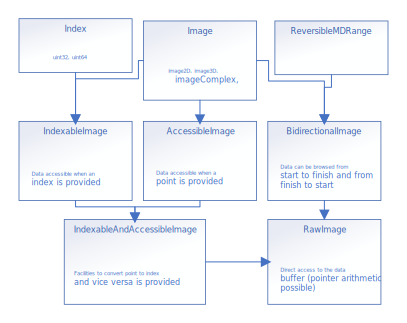
\includegraphics[width=.8\linewidth]{../figures/concepts/images_all}
  \caption{All images concepts.}
  \label{fig:concept.images}
\end{figure}


\subsection{Local algorithm concepts: structuring elements and extensions}
\label{subsec:local.se.ext}

From the beginning concepts are emerging from behavioral patterns extracted from algorithms. In image processing, there
is a family of algorithms called the \emph{local algorithms}. They work by considering a specific pixel as well as all
the pixels among a window having a specific shape centered in this first pixel. The window is called the
\emph{structuring element} and the pixels considered by this window are called the \emph{neighborhood}. This leads us to
introduce the concept of \emph{StructuringElement} which is defined in~\cref{table:concept.se.definitions}.

This concept is refined into three sub-concepts that are related to properties the structuring element can offer. Those
properties are:
\begin{itemize}
  \item decomposability: ability to split a complex structuring element into several smaller and simpler structuring
        element. There is an equivalence in behavior when the algorithm is recursively run for each smaller structuring
        element one after another, in a multi-pass way.
  \item separability: ability to split a complex structuring element into several smaller and simpler structuring
        element. There is an equivalence in behavior when the convolution is recursively run for each smaller
        structuring element one after another, in a precise order, in a multi-pass way.
  \item incremental: ability to tell the points that are added to or removed from the range when the structuring element
        is shifted by a basic displacement (e.g. for a \emph{2D point}, the basic displacement is \((0,1)\)). Usually
        used to compute attributes over a sliding structuring element in linear time.
\end{itemize}

\FIXME{Give examples}

The behavioral for those concepts is described in~\cref{table:concept.se.expressions}. Being able to manipulate
structuring element allows us to write the following code:
\begin{minted}{C++}
  auto se = se::disc(.radius=3); // get a structuring element
  for(auto pix : ima.pixels())   // traverse image
    for(auto nb : se(pix))       // traverse neighboring pixels
      // ...
\end{minted}

Additionally, we introduce the concept of \emph{Neighborhood} in~\cref{table:concept.nbh.definitions}. This concept has
facilities to know what points/pixels are placed before or after another point/pixel inside the window of a specific
structuring element. It behaves as described in~\cref{table:concept.nbh.expressions}. This concept is useful when one
wants to only consider a certain part of the neighboring pixels within a structuring element. This offers the
opportunity to write the following code:
\begin{minted}{C++}
  auto se = se::disc(.radius=3); // get a structuring element
  for(auto pix : ima.pixels())   // traverse image
    for(auto nb : se.before(pix))// traverse neighboring pixels located before pix
      // ...
\end{minted}

And the last concept we need to introduce is the extension. Indeed, extension management is very important when dealing
with local algorithm as pixels on the border need to be processed too, and the behavior near the border of the image
must be defined and well-specified. There are several strategies when it comes to borders and extension. We refine
concept for each strategy we identified:
\begin{itemize}
  \item \emph{fillable}: fill the border with a specific value.
  \item \emph{mirrorable}: mirror the image as if there was an axial symmetry, with the border being the axis.
  \item \emph{periodizeable}: repeat the image, as if a modulo size was applied to the coordinates.
  \item \emph{clampable}: extend the value at the image's border into the extension.
  \item \emph{extent\_with}: used when tiling. It considers the current image as a sub-image of another bigger image and
        pick the extension values there.
\end{itemize}
Those concepts are defined in~\cref{table:concept.extensions.definitions} and their behavior is described
in~\cref{table:concept.extensions.expressions}. All those concepts allow us to introduce the final refined image
concepts: \emph{WithExtensionImage} as well as \emph{ConcreteImage} and \emph{ViewImage}. Those two last will be seen in
detail in the next~\cref{chap:image_views}. Those concepts are defined in~\cref{table:concept.image.definitions.7}.
Their behavior is described in~\cref{table:concept.image.expressions.7}. It is now possible to write the following code:
\begin{minted}{C++}
  template <class I, class SE>
  my_local_algorithm(I input, SE se) {
    // if the extension is large enough to function with the passed structuring element
    if(input.extension().fit(se)) {
      // ...
    }
  }
\end{minted}

We show how those three concepts (structuring elements, neighborhood and extension) interact with each other in the
diagram shown in~\cref{fig:concept.se_extension}.

\begin{figure}[htbp]
  \centering
  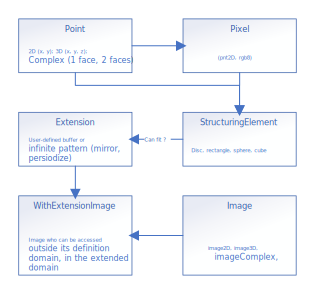
\includegraphics[width=.8\linewidth]{../figures/concepts/se_extension}
  \caption{Structuring element and Extension concepts.}
  \label{fig:concept.se_extension}
\end{figure}

Finally, we introduce a helper concept to centralize the detection of the ``writability'' of an image. Indeed, we do not
want the user to have to use the writable counterpart of each concept for each and every case. That is why we introduce
this final concept, \emph{OutputImage} in~\cref{table:concept.image.expressions.8}, that will tell the user if an image
is well-specified.

The correct way to use it is:
\begin{minted}{c++}
template <class Img>
requires RawImage<Img> && OutputImage<Img>
void my_algorithm(Img img) {
    // write data in img ...
  }
\end{minted}

\section{Summary}

In this chapter, we present that concepts are not designed after data structures but after algorithms. Indeed, a concept
consists in extracting a consistent behavioral pattern from a piece of code (algorithm) and name it to give him a
meaning. Through a simple but concrete example, we present in a didactic way how to extract concepts from an image
processing algorithm (gamma correction).

This chapter then proceeds to explain how, in theory, image types are related to each other. We present the set of
different image types and how algorithms exist in those sets, which introduce the notion of \emph{version} of an
algorithm. An algorithm will have different \emph{versions} for each image types set it supports. We distinguish it from
an algorithm \emph{specialization}, the latter being the ability to use an opportunity (related to a property) to make
an optimization and increase performances.

This chapter then proceed to describe the notion how algorithm canvas which is the result flowing from the taxonomy of
image processing algorithms. Indeed, there are three main algorithm families: the pixel-wise algorithms (binary
threshold), the local algorithms (dilation) and the global algorithms (Chamfer distance transform). We focus primarily
on local algorithms and how they can all be written through the same canvas of code. Indeed, for instance, the only
difference between a dilation and an erosion is the operator (max vs. min). We then discuss ways to exploit these canvas
to possibly solve heterogeneous computing issues.

Finally, this chapter introduces our first main contribution: a complete taxonomy related to the image processing area.
We first introduce fundamental concepts such as \emph{point}, \emph{pixel}, \emph{domain} and \emph{image}. We then
motivate and introduce advanced concepts related to images and the different way to access data (forward, backward
traversing, indexing, direct access to underlying buffer, \ldots). In the end, we introduce the concepts related to
orbiting notions such as \emph{structuring element}, \emph{neighborhood} and \emph{extension} (border management) which
are necessary to be able to work with local algorithms.

The next chapter will make use of the presented concepts to introduce the second main contribution of this thesis: the
\emph{image views}.
